\chapter{Background}

\section{Software engineering}

\todo{emergence of SE}
The craft of software engineering emerged during the 1960s. Software crisis, the growing cap between expectations and results for software, called for a more systematic approach to software production \cite{mcclure_nato_1968}. Authors suggested that software should be considered a branch of engineering, like hardware. NATO-organized conference in 1968 widely launched the new, engineering-inspired approach to software production.

\todo{defining SE}
Even though the comparison to engineering was initially used to provoke thought \cite{mcclure_nato_1968}, it has since established as a part of the software production vocabulary, although the concept of software engineering has remained a topic of dispute in academia. Boehm \cite{boehm_software_1979} leans to the Webster dictionary definitions for software and engineering, combining them to a formal definition of software engineering: applying science to create "useful to man" computer programs and documentation. He argues that the difference between arbitrary development and software engineering is that the latter ensures the end result is indeed useful for the end-users, therefore satisfying the specification.  Sommerville on the other hand establishes the gap between software development and software engineering: he defines software development as the actual development process where code is written, whereas software engineering is tied to the life cycle of the software – from planning to maintenance. \cite{sommerville_software_2016}

Both the engineering mindset and the lifecycle of the software are included in IEEE's take on software engineering. The definition can be described as a combination of Boehm's and Sommerville's definitions. For the purpose of this thesis, we will be using this definition. \cite{noauthor_ieee_1990}

\subsection{Software development life cycle}

Software engineering can be divided into four main activities: software specification, software development, software validation and software evolution. \cite{sommerville_software_2016} These steps can also be called a software process or a software development life cycle (SDLC). Commonly used SDLCs include Waterfall model, Validation \& Verification model (V model) and Agile methods. \cite{balaji_waterfall_2012} Projects can benefit from different approaches: dimensions such as level of risk, budget or project timeline vary between the SDLCs. \cite{alshamrani_comparison_2015, cohen_introduction_2004} 

- A trend towards iterative methods can be seen in the industry (sommerville) 

\subsubsection{Waterfall model}

The Waterfall model is widely referred as the most well-known SDLC. Waterfall model consists of 5 sequential process stages: requirements analysis, design, coding, testing and maintenance. \cite{alshamrani_comparison_2015} The name implies that a project following Waterfall model is one-way: like water, it moves only forwards and different stages don't overlap. Each stage produces an deliverable to be used as a basis on the upcoming stage: for example, \textit{lorem ipsum lorem ipsum lor}~\cite{balaji_waterfall_2012}

In practice though, projects rarely follow Waterfall model in a blindly manner: upcoming stages are prepared in parallel to the current one, and previous stages are revisited when the need arises. \cite{sommerville_software_2016}

A significant shortcoming of Waterfall model is that the software is only delivered once, in the end of the project. 

- real life example of safety- / mission-critical software?
- good if cost of change is high or requirements are very well known and fixed
- problems with traditional methods that have driven agile methods (introduction to agile) 
- look up the original waterfall paper, mentions also "agile" methodology

\subsubsection{Agile methods}

Agile methods is an umbrella term that includes methodologies like Extreme Programming, Lean Development and Scrum. The terminology is further complicated due to the improper usage of the term in the industry. The common properties of Agile methods include iterative development, focus on communication and the critical stance toward intermediate deliverables like requirements. Furthermore, Agile evangelists have agreed that Agile is more about "state of mind" rather than a single process or methodology. \cite{cohen_introduction_2004}

In iterative development, new versions of working product are delivered constantly: most productive teams deploy software to production even multiple times in a day \cite{forsgren_accelerate_2018}. This enables the end-users to use the software from early days of the development cycle. Development teams are able to receive constant feedback from users and iterate the software accordingly for the next releases. \cite{balaji_waterfall_2012}

Focus on communication encourages development teams to enable low-threshold, constant communication practices instead of documentation-heavy decision-making methods. Agile methods introduce practices like daily stand-up meetings and pair programming to support this. When Agile methods emerged, co-locating team members was also seen as a key to success for working communication. With the possibilities presented by modern collaboration platforms like Slack and Zoom, low threshold communication has become possible for remote teams – working from the same physical location is no longer seen as crucial for Agile implementation.

Another definitive characteristic of Agile methods is the critical stance toward intermediate, non-critical deliverables. By reducing the resources spent on these artifacts, teams can focus their efforts on the development of the product. \cite{cohen_introduction_2004} The self-managing nature of Agile teams further promotes the idea that the team has the best context to prioritize and plan their work. \cite{alshamrani_comparison_2015} 

Even though Agile has an evergrowing status in the software development world, traditional methods like Waterfall are still needed. Large teams and complex projects are seen as environments where more structured processes should be preferred. On the other hand, teams are increasingly incorporating Agile properties into their traditional software processes and vice versa. \cite{cohen_introduction_2004} 

\subsection{DevOps}

Agile has transformed the way software is developed. But, in the software lifecycle, the performance of testing, deployment and post-deployment functions like fault recovery should be considered. DevOps brings development and IT operations closer together, bridging the gap between these silos and enabling agileness throughout the lifecycle of the software \cite{hemon-hildgen_agile_2020}. DevOps aims to shorten the software development life-cycle by introducing automated tools that ship code to production faster, boosting both productivity and quality of development\cite{cois_modern_2014}. According to Humble and Molesky, DevOps practices can be devided to four main aspects: automation, culture, sharing and measurement\cite{humble_why_2011}. 

\todo{automation on devops}
Most distinctive automation practices introduced by DevOps are continuous integration (CI) and continuous delivery (CD). In continuous integration, changes made by the developers are often submitted as soon as possible back to the main branch, usually preceded by a build task and automated unit tests run by a CI worker. CI is often followed by CD, which is in charge of integration testing, end-to-end testing and finally deploying the approved version into a staging environment. The abbreviation "CD" is commonly also used to refer to continuous deployment. 

In addition to the steps included in continuous delivery, continuous deployment automates the deployment of software to production environments. In contrast, continuous delivery pipelines require the user's manual interaction to initialize deployments. In the industry, CD usually refers to continuous delivery, though the term is used in quite liberal manner. Systems consisting of both CI and CD functions are called the CI/CD pipeline. In modern-day DevOps, having a stable CI/CD pipeline in place is seen as a backbone to the success of the team. 

\todo{culture on devops}
In addition to concrete tools, DevOps is about ways of working. Socio-technical factors have to be taken into consideration to truly create a well-functioning DevOps function \cite{hemon-hildgen_agile_2020}. 

\todo{sharing on devops}

\todo{measurement on devops}
- process improvement -> process measurement -> developer productivity?

\section{Developer productivity}

\subsection{Productivity in general}
\todo{traditional productivity and productivity in knowledge work}
Productivity in industrial engineering is defined as the ratio of input and output\cite{syverson_what_2011, chew_no-nonsense_1988}. In manufacturing, input and output are relatively easily measured as the used resources and the produced goods. On the other hand, non-manufacturing businesses rely on more complex definitions: in knowledge work, man-hour is not considered as a relevant metric of productivity \cite{tangen_demystifying_2005}. The definition of output has also been under debate. In 1988, Chew presented a view that output should include other metrics than "number of units", for example quality, timeliness and price of the product \cite{chew_no-nonsense_1988}. Many relatively similar, context definitions have also emerged in the literature \cite{tangen_demystifying_2005}.

\todo{definition of performance and productivity}
The terms productivity and performance are sometimes used interchangeably. To further complicate the terminology, authors define performance as a component of productivity and vice versa. Based on vast amount of literature research, Tangen defines performance as "umbrella term of excellence", consisting of productivity and other non-cost elements, whereas productivity itself is defined as "physical phenomenon" – the ratio of input and output \cite{tangen_demystifying_2005}. As an example of the opposite approach, SPACE authors define performance as "outcome of a system or process", measured by metrics like service health or customer satisfaction. Productivity in the SPACE framework is about the sum of it's parts, performance representing one of five \cite{forsgren_space_2021}. To sum things up, these terms are used to refer to varying phenomenons in different situations.

\todo{productivity in different contexts}
In the examples before, productivity is reviewed from the company's perspective. Often it is beneficial to look into the metrics of a smaller entity: a department, a team or an individual \cite{forsgren_space_2021, tangen_demystifying_2005}. These metrics can be used to provide more accurate insights of the entity in question.

\todo{measuring productivity, how to choose metrics}
When measuring productivity of teams or individual employees, it can be tempting to incentivize them based on the metrics. For example, software developers could get promotions or raises if they contribute more-than-average to the product. Often these ambitions can lead to unwanted results as employees start to optimize their work to meet the metric, rather than what would be best for the company\cite{symons_software_2010, chew_no-nonsense_1988}: if the metric would be amount of pull requests, it would be tempting to break the work to very small increments to pump up the numbers. Individual preferences further difficult the topic, as some employees by habit contribute more commits than others \cite{oliveira_code_2020}. 

\subsection{Productivity in software engineering}

Determining the productivity of engineers is seen crucial for the success of software development. Therefore, a substantial amount of research has been concluded on this subject in the past years.\cite{oliveira_code_2020}

No consensus has been found on how to measure productivity accurately. Historically, source code based metrics such as lines of code or amount of commits have been utilized\cite{oliveira_code_2020}. Nowadays these metrics are considered, at best, a vague representation of the true productivity \cite{forsgren_space_2021}.

Modern frameworks have explored the work of an software engineering team as a joint effort: as popular SDLCs put emphasis on teamwork, the productivity should be assessed in the same context. The team is seen as the "basic work unit" \cite{moe_overcoming_2010} and the research has shifted towards how teams can improve together. Even though super-performing individuals are still seen as valuable asset, companies should focus their efforts on building and enabling super-performing teams \cite{forsgren_space_2021}. 

Agile methods use velocity – units of completed work in time frame – to measure productivity. Although velocity is considered as a better indicator of productivity than source code metrics, it has major drawbacks as pointed out by Forsgren et al. in their industry-shaping book Accelerate. Most importantly, velocity is a highly relative to the context and can't be used as an absolute metric. Secondly, velocity is a good example of a metric that is prone to be gamed by the employees, as described previously.\cite{forsgren_accelerate_2018}
 
\subsection{Developer productivity frameworks}

- common characteristics of frameworks
- why are these needed

\todo{DORA metrics}

DevOps Research and Assessment (DORA), a Alphabet Inc subsidiary, has pioneered the research of DevOps and developer productivity. In their book Accelerate, they presented "four key metrics" to measure software delivery performance, often referred to as the DORA metrics. The metrics are as follows: 

\begin{enumerate}
\item Lead Time
\item Deployment Frequency
\item Mean Time to Restore
\item Change Fail Percentage
\end{enumerate}

\todo{Lead Time}
Lead Time is a metric derived from Lean manufacturing to software world. In essence, Lead Time refers to the time from a feature request to the change that fulfills the request. Often in software, the changes are not directly requested by single customers, but rather decided by the teams using input from stakeholders. DORA metrics define Lead Time as the time from commit to code running in production environment \cite{forsgren_accelerate_2018}.

In this thesis, we use Lead Time to refer to the time from the first commit to a new branch to the moment it is merged to the main branch, as seen in figure \ref{fig:CycleTime}. The industry term for this metric is Pull Request Cycle Time. 

\begin{figure}[ht]
    \begin{center}
        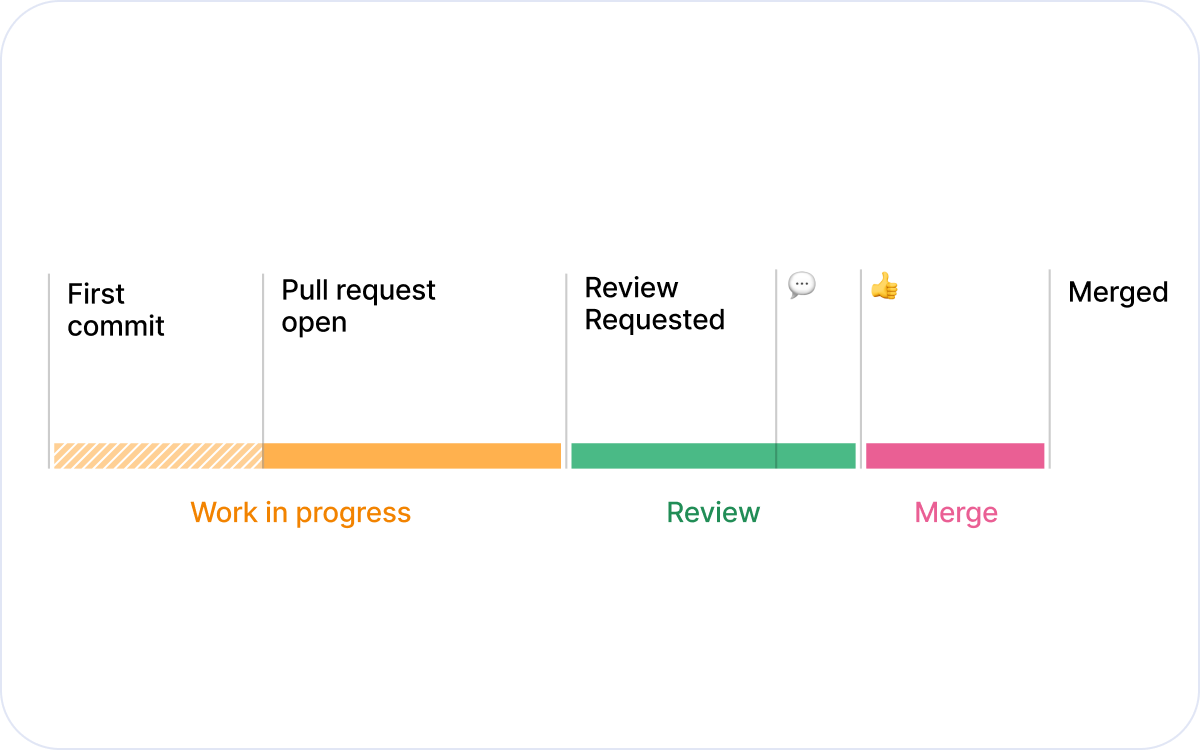
\includegraphics[width=13.5cm]{images/cycletime_defined}
        \caption{Pull Request lifecycle \cite{swarmia_reducing_nodate}}
        \label{fig:CycleTime}
    \end{center}
\end{figure}

\todo{Deployment Frequency}
Originally in Toyota production system, batch size was used as a key performance metric. DORA researchers note that in the software development context, batch size is a sub-optimal metric. They have therefore used Deployment Frequency as a proxy to estimate batch size. Deployment Frequency is defined as the frequency of pushing a new version to the production environment.  

\todo{Mean Time to Restore and Change Fail Percentage}
Both Lead Time and Deployment Frequency are metrics for the "software delivery performance tempo". To determine if the increase in tempo has disadvantages in terms of software quality or system stability, two additional metrics are used: Mean Time to Restore and Change Fail Percentage. Both of these measure situations where the production system has failed for some reason. The authors articulate that as in rapidly changing software systems failure is a common situation, the absolute amount of failures is an obsolete metric. Rather, they find that the time taken to restore the service or application after a incident takes or how large percentage of changes lead to a production system failure. 

\todo{further justification of DORA metrics}
In Accelerate, the results are clear: increasing software delivery tempo has no negative impact on the stability or quality. Instead, teams that perform well in the first two metrics also had better results in the rest measures. 

\todo{SPACE Framework}

- space builds on dora, what are the major additions
- what is the relevance here

\section{Software engineering as teamwork}

Work is often organized around teams. To distinguish team from other groups that work together, we use definition by Katzenbach & Smith: "team is a small number of people with complementary skills who are committed to a common purpose, set of performance goals, and approach for which they hold themselves accountable" \cite{katzenbach_discipline_1993}. The fundamental difference is the accountability, on both individual and team level: team members are primarily responsible for each othedanr, their supervisors or other stakeholders \cite{katzenbach_discipline_1993}.

In software engineering, teams work together to design, develop and maintain products. Working as a team offers upsides such as increased employee satisfaction, innovation and productivity \cite{moe_teamwork_2010}. The team is considered as the "basic work unit", rather than the individual \cite{moe_overcoming_2010}. This has motivated companies and executives to focus on building hyper-performing teams.

The toolbox for leadership to enable teams full potential includes: A B C

\subsection{Self-managing teams}

Modern software development methods encourage, or even require, usage of self-managing teams \cite{moe_teamwork_2010}. Other terms used to define the phenomena include self-organizing team, autonomous team and empowered team. Even though majority of studies report that forming self-managing teams lead to positive outcomes, there has also been opposing conclusions. Factors such as insufficient leadership or nature of the situation can lead to the difficulty of implementation of such team \cite{moe_teamwork_2010}. 

\todo{leaderships role in self-managing teams}
To enable true self-management in a team, leadership and other internal stakeholders have to respect their independence and improvement efforts \cite{moe_overcoming_2010}. 

\todo{team norms}
To improve, self-managing teams have to change their behavior, either by self-managing or from an external stimulus. Teams that are able to self-improve can achieve more autonomy than their counterparts. Norms, standards that regulate team members behaviors, are of essence when building a productive software development team \cite{abrahamsson_exploring_2016}. Norms can include both technical and non-technical rules: for example, teams can commit to test-driven development or to promoting pair programming. The impact of norms for development teams is achieved through increased simplicity of common processes: team members can trust that their colleagues do certain activities and refrain from the unwanted ones \cite{abrahamsson_exploring_2016}. 

Team norms can form in two ways: either by organically within the team or by others, or as part of organization's guidelines or direct influence \cite{teh_social_2012}. 

- potential tools/solutions
-> linking to chapter 3